%%%%%%%%%%%%%%%%%%%%%%
% INTRODUCTION TO THE COALESCENT
%%%%%%%%%%%%%%%%%%%%%%

\begin{frame}
\frametitle{The coalescent}

Data: a \alert{small genetic sample} from a \alert{large background population}.

\smallskip 
\alert{The coalescent }
\begin{itemize}
\item is a model of the ancestral relationships of a sample of individuals taken from a larger population.
\smallskip
\item describes a probability distribution on ancestral genealogies (trees) given a population history, $N(t)$. 
  \begin{itemize}
	\item Therefore the coalescent can convert information from ancestral genealogies into information about population history and vice versa.
  \end{itemize}
\smallskip
\item a model of ancestral genealogies, not sequences, and its simplest form assumes neutral evolution.
\smallskip
\item can be thought of as a prior on the tree, in a Bayesian setting.
\end{itemize}

\end{frame}

\begin{frame}
\frametitle{Theoretical population genetics}

\begin{columns}

\column{.64\textwidth}

Most of theoretical population genetics is based on the idealized
Wright-Fisher model of population which assumes

\begin{itemize}
\item Constant population size $N$
\item Discrete generations
\item Complete mixing
\end{itemize}
For the purposes of this presentation the population will be assumed to be haploid,
as is the case for many pathogens. 


\column{.36\textwidth}

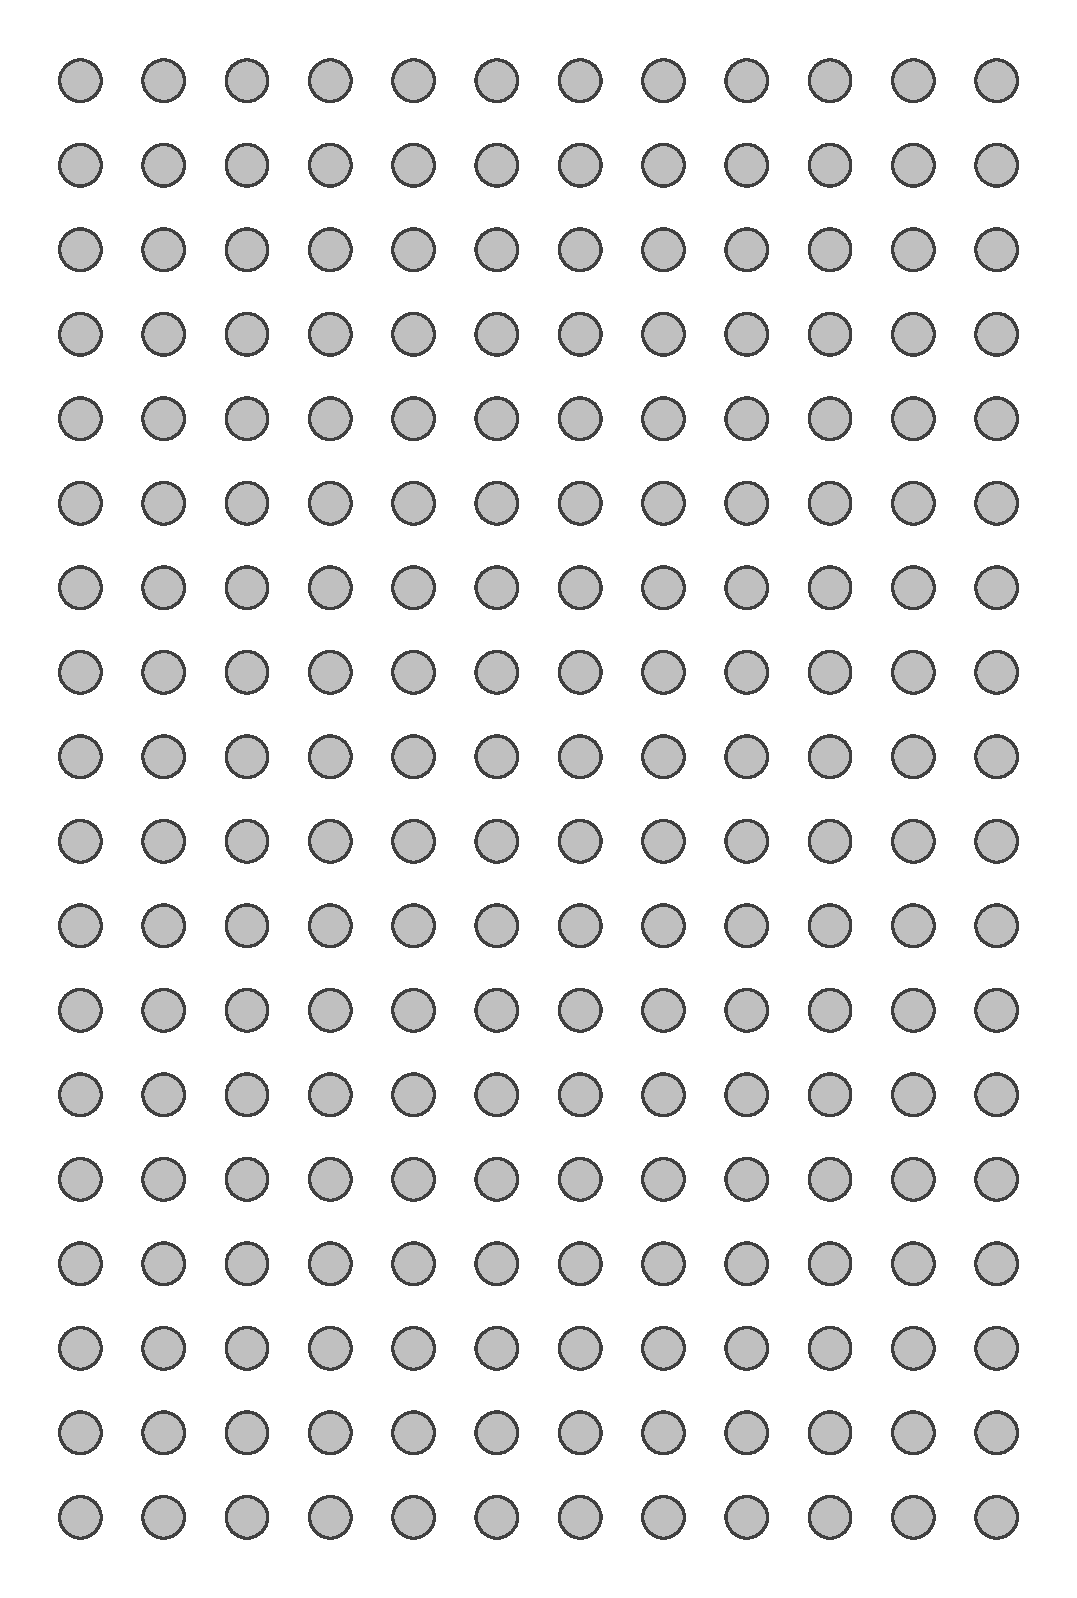
\includegraphics[scale=0.25]{../images/wrightFisher}

\end{columns}

\end{frame}


%\begin{frame}
%\frametitle{Some classical neutral results for ideal populations}

%\begin{columns}

%\column{.6\textwidth}

%\begin{itemize}
%\item The probability of fixation of a novel, neutral mutation is $\frac{1}{N}$
%\item The average time to this fixation is approximately $2N$ generations
%\item Again, assuming neutral mutations, the average number of mutations between
%a random pair of individuals from the same generation is 
%\end{itemize}
%\begin{equation}
%\Theta=2N\mu\,.\end{equation}

%
%%\begin{itemize}
%%\item Another way of saying this is that the average number of mutations
%%back to the common ancestor of two random individuals is $N\mu$.
%%\end{itemize}

%\column{.4\textwidth}

%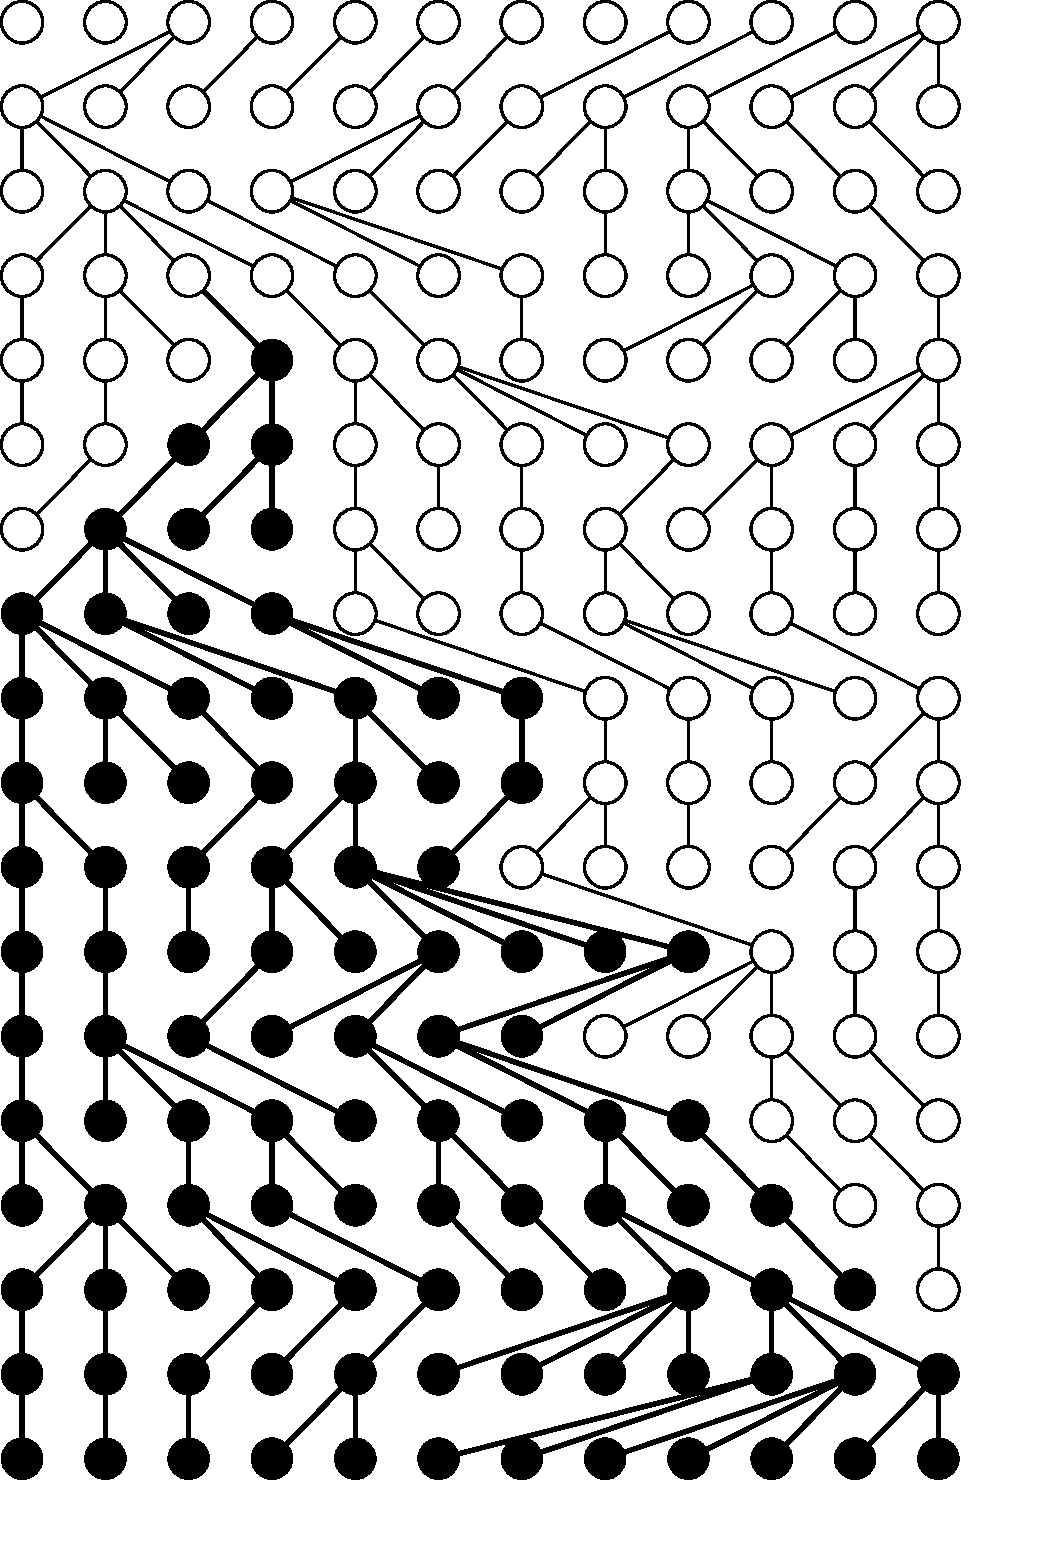
\includegraphics[scale=0.25]{../images/wrightFisherNovelMutant}

%\end{columns}

%\end{frame}


\begin{frame}
  \frametitle{Kingman's n-coalescent}

\begin{columns}

\column{.64\textwidth}

Consider tracing the ancestry of a sample of $k$ individuals from the present,
back into the past.

This process is a discrete-time Markov process that eventually \emph{coalesces} to a
single common ancestor (\emph{concestor}) of the sample of individuals. 

Kingman's n-coalescent is a \emph{continuous-time}  diffusion approximation of this process, in the limit
of large $N$, i.e. $N \gg k^2$.

\column{.36\textwidth}
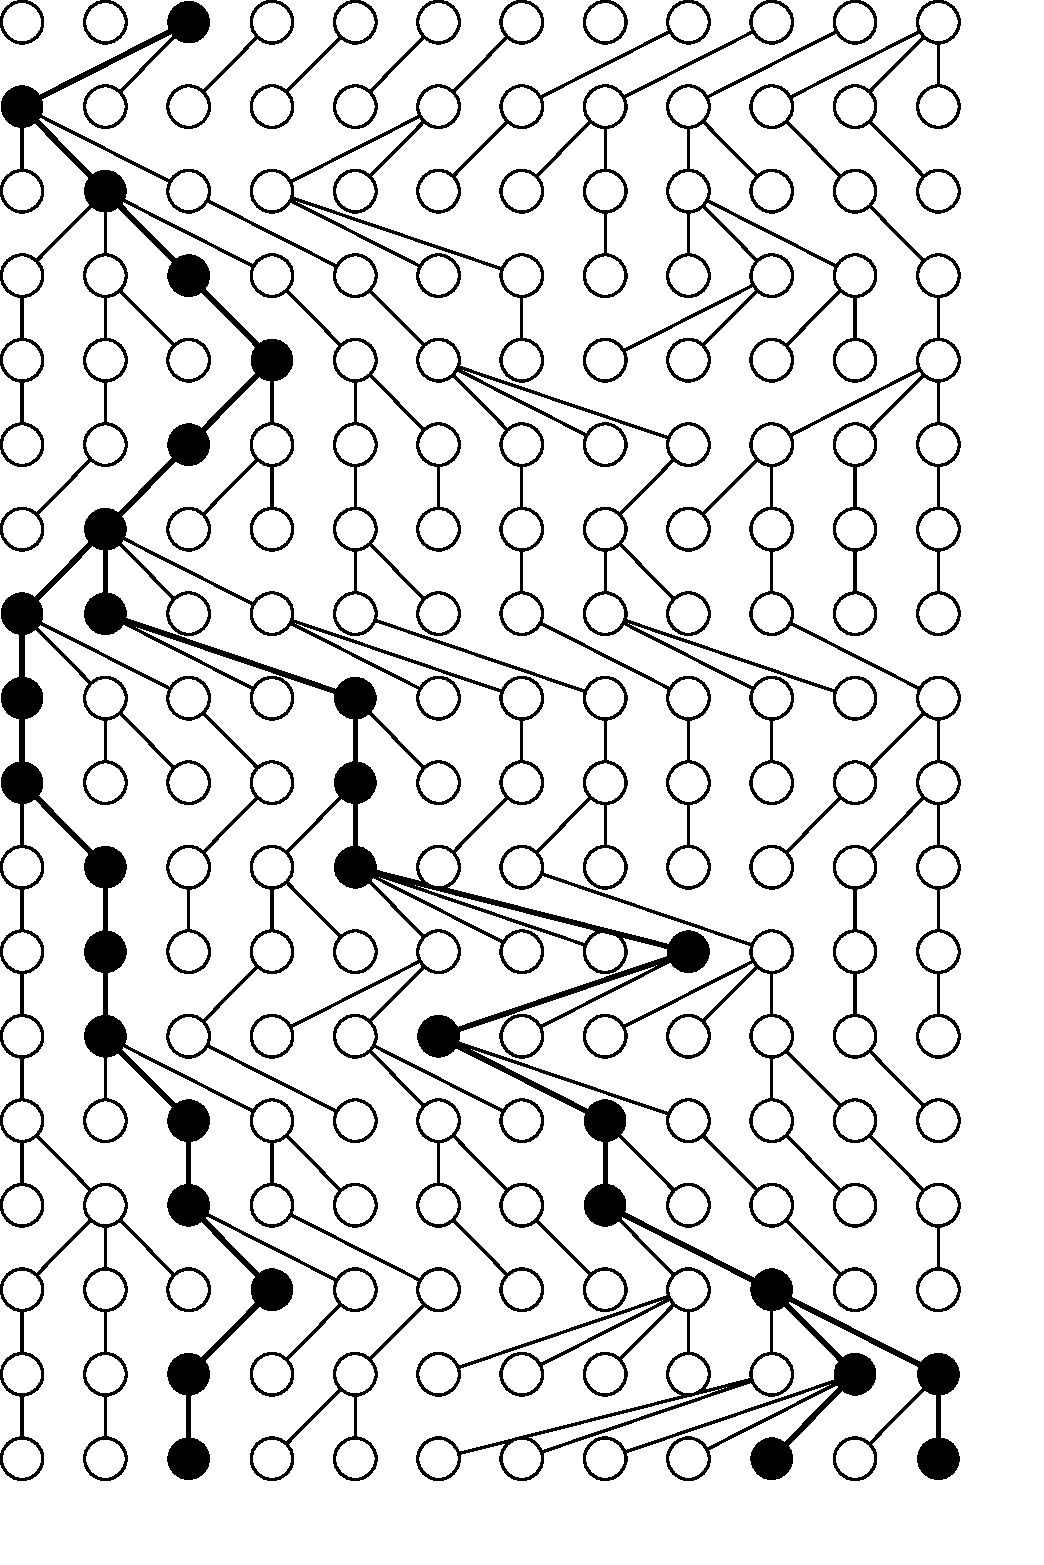
\includegraphics[scale=0.25]{../images/wfCoalescent3}

\end{columns}

\end{frame}

\begin{frame}
\frametitle{The coalescence of two ancestral lineages}

\begin{columns}

\column{.64\textwidth}

\begin{itemize}
\item First, consider two random members from a population of fixed size $N$. 

\item By perfect mixing, the probability they share a \emph{concestor} in the previous generation is $1/N$. 

\item The probability the concestor is $t$ generations back is 

\begin{equation*}
Pr\{t\} = \frac{1}{N}(1-\frac{1}{N})^{t-1}. 
\end{equation*}

\item It follows that $g=t-1$, has a geometric distribution with a success rate of $\lambda =
1/N$, and so has mean $N$ and variance of $N^3/(N-1)$.
\end{itemize}

\column{.36\textwidth}
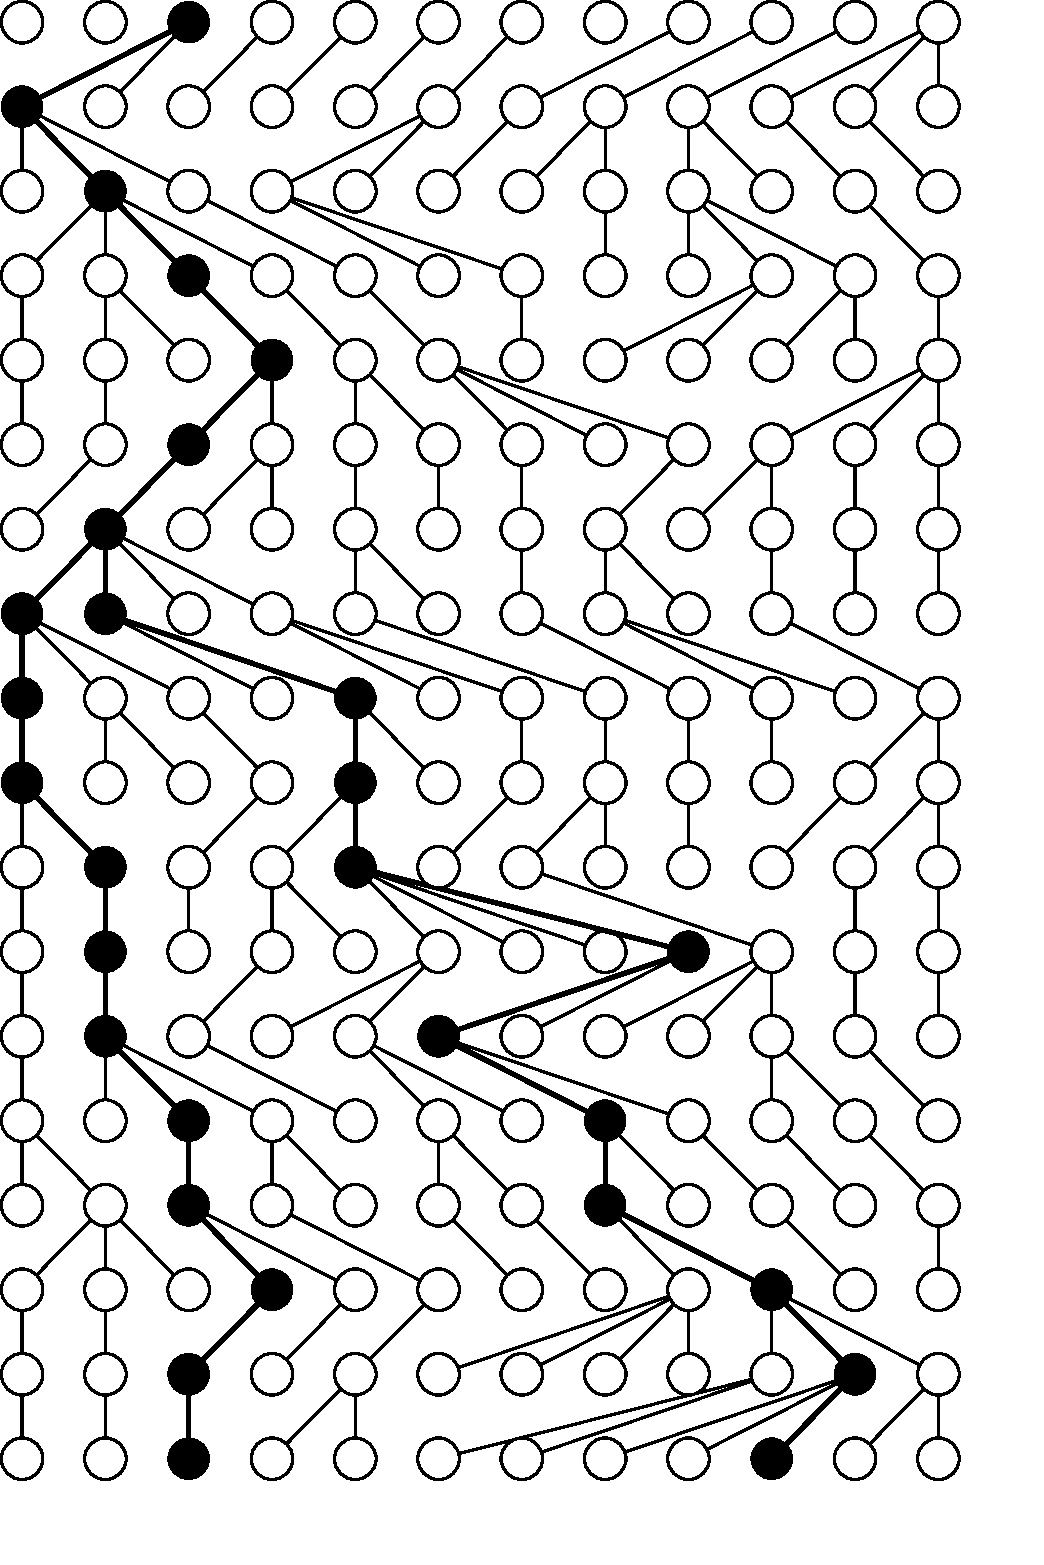
\includegraphics[scale=0.25]{../images/wfCoalescent2}

\end{columns}

\end{frame}

\begin{frame}
\frametitle{The coalescence of $k$ lineages}

\begin{columns}

\column{.64\textwidth}

With $k$ lineages the time to the first coalescence is derived in the same way,
only now there are $\binom{k}{2}$ possible pairs that may coalesce, resulting in
a success rate of $\lambda = \binom{k}{2}/N$ and mean time to first coalescence ($t_k$) of

\begin{equation*}
E[t_k] = \frac{N}{\binom{k}{2}}.
\end{equation*}

This implicitly assumes that $N$ is much larger than $O(k^2)$, so that the probability
of two coalescent events in the same generation is small.


\column{.36\textwidth}
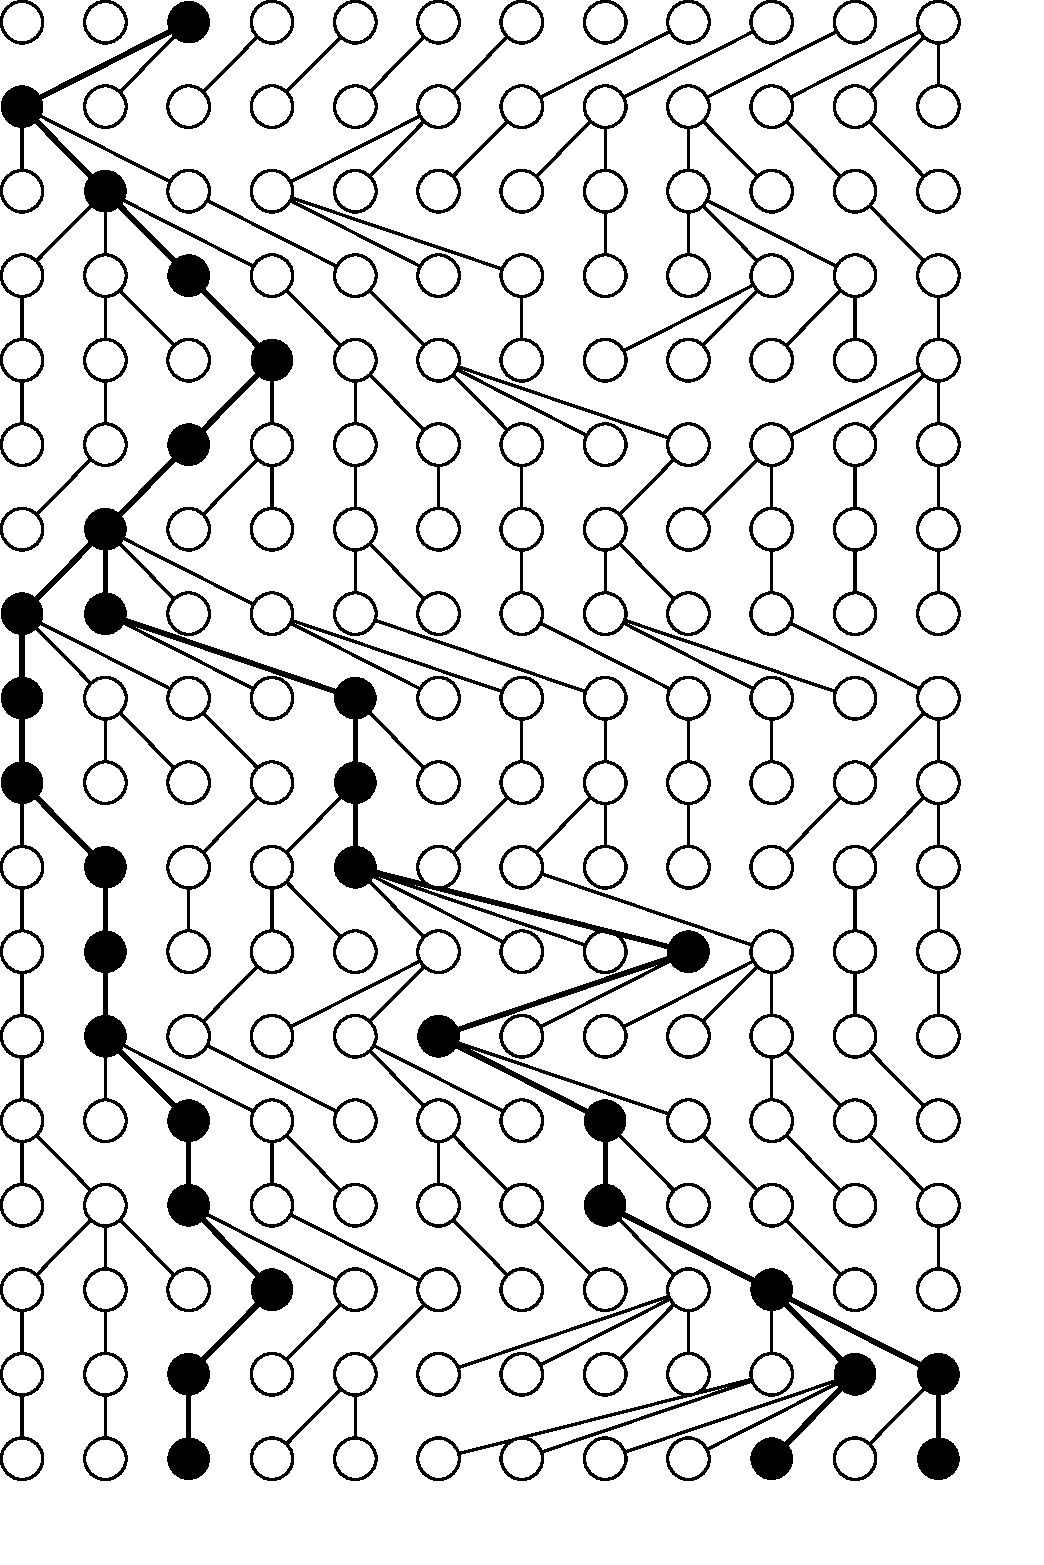
\includegraphics[scale=0.25]{../images/wfCoalescent3}

\end{columns}

\end{frame}


%\begin{frame}
%\frametitle{Some classical coalescent results}

%An interesting consequence is that the average number of generations required for all $k$ lineages to
%coalesce into one is 

%\begin{equation}
%E[t_{root}] = \sum_{i=2}^k \frac{N}{\binom{i}{2}} = 2N(1-\frac{1}{k}), 
%\end{equation}

%which approaches $2N$ as $k$ increases.

%\end{frame}


\begin{frame}
\frametitle{The coalescent is a \emph{diffusion approximation}}

Kingman (1982) showed that as $N$ grows the coalescent process converges to a
continuous-time Markov chain.

\medskip
\begin{columns}[t]

\column{0.5\textwidth}

$\lambda = \binom{k}{2}/N$ is the rate of coalescence, i.e. the probability of coalescing a pair from $k$ lineages on a short time
interval $\Delta t$ is $O({\lambda\Delta t})$. Unsurprisingly the solution turns
out to be the exponential distribution:

\column{0.5\textwidth}

%\center{
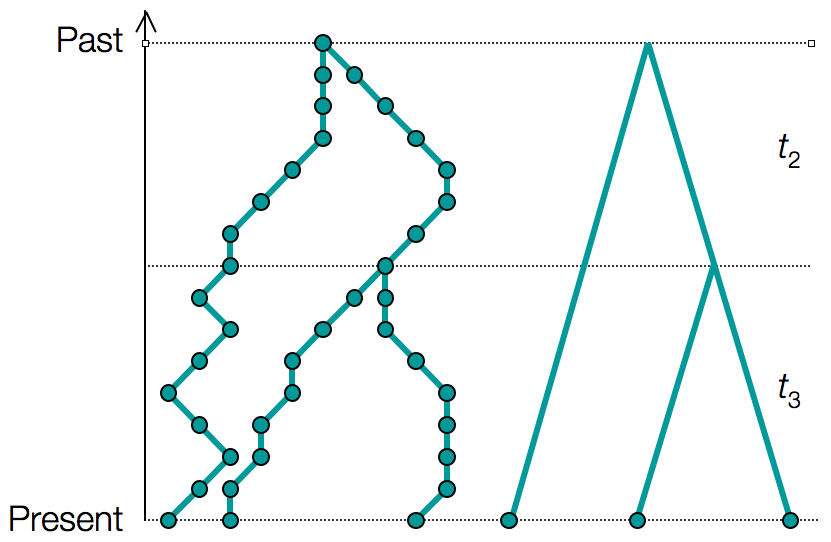
\includegraphics[scale=0.18]{../images/wrightFisherToTree}

%{\small{discrete versus continuous}}
%}

\end{columns}

\bigskip

\begin{equation*}
f(t_k)=\frac{{k \choose 2}}{N}\exp\left(-\frac{{k \choose 2}t_k}{N}\right)\,.
\end{equation*}

\end{frame}

\begin{frame}
\frametitle{The coalescent density for a genealogy}

For a genealogy with coalescent times $\mathbf{t}=\{t_2, t_3, ..., t_n\}$ we can write the probability density, given $N$:

\begin{equation*}
f(\mathbf{t}|N)=\frac{1}{N^{n-1}}\prod_{k=2}^n\exp\left(-\frac{{k \choose 2}t_k}{N}\right)\,.
\end{equation*}

\center{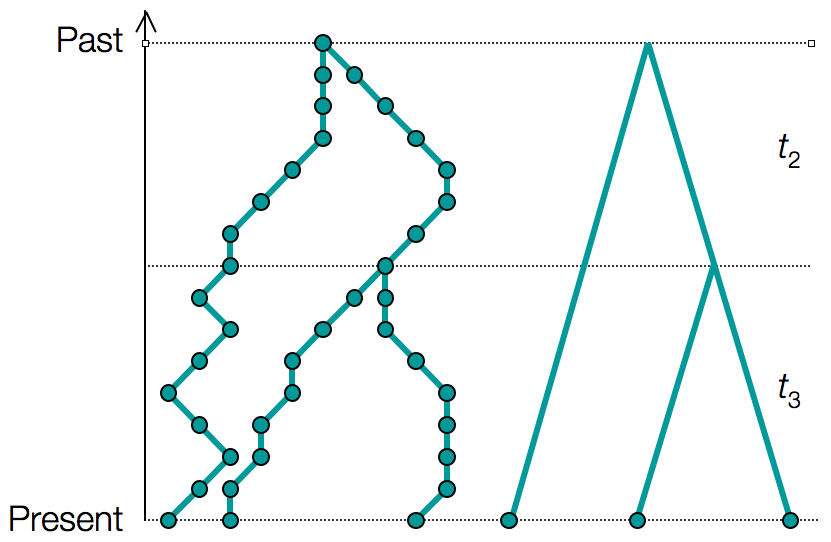
\includegraphics[scale=0.22]{../images/wrightFisherToTree}}

\end{frame}

\begin{frame}
\frametitle{The coalescent density with varying population size}

The generalization of the coalescent for the case where the
population size changes over time, $N = N(t)$ is given by Griffiths and Tavare (1994). They showed that the coalescent density for the first coalescence event being at time $t$ in the past given $n$ lineages is:

\begin{equation*}
f(t) = {\frac{1}{N(t)}}  
{\exp\left(-{\int \limits_0^t \frac{\binom{n}{2}}{N(x)} dx }\right)} 
\label{coalescent-density-with-nt}
\end{equation*}

\end{frame}

\begin{frame}
\frametitle{The coalescent with serial samples}

Many epidemiological agents, like RNA viruses, evolve very rapidly, so that the effect of sampling the population at different times becomes important.

\begin{columns}[t]

\column{0.5\textwidth}

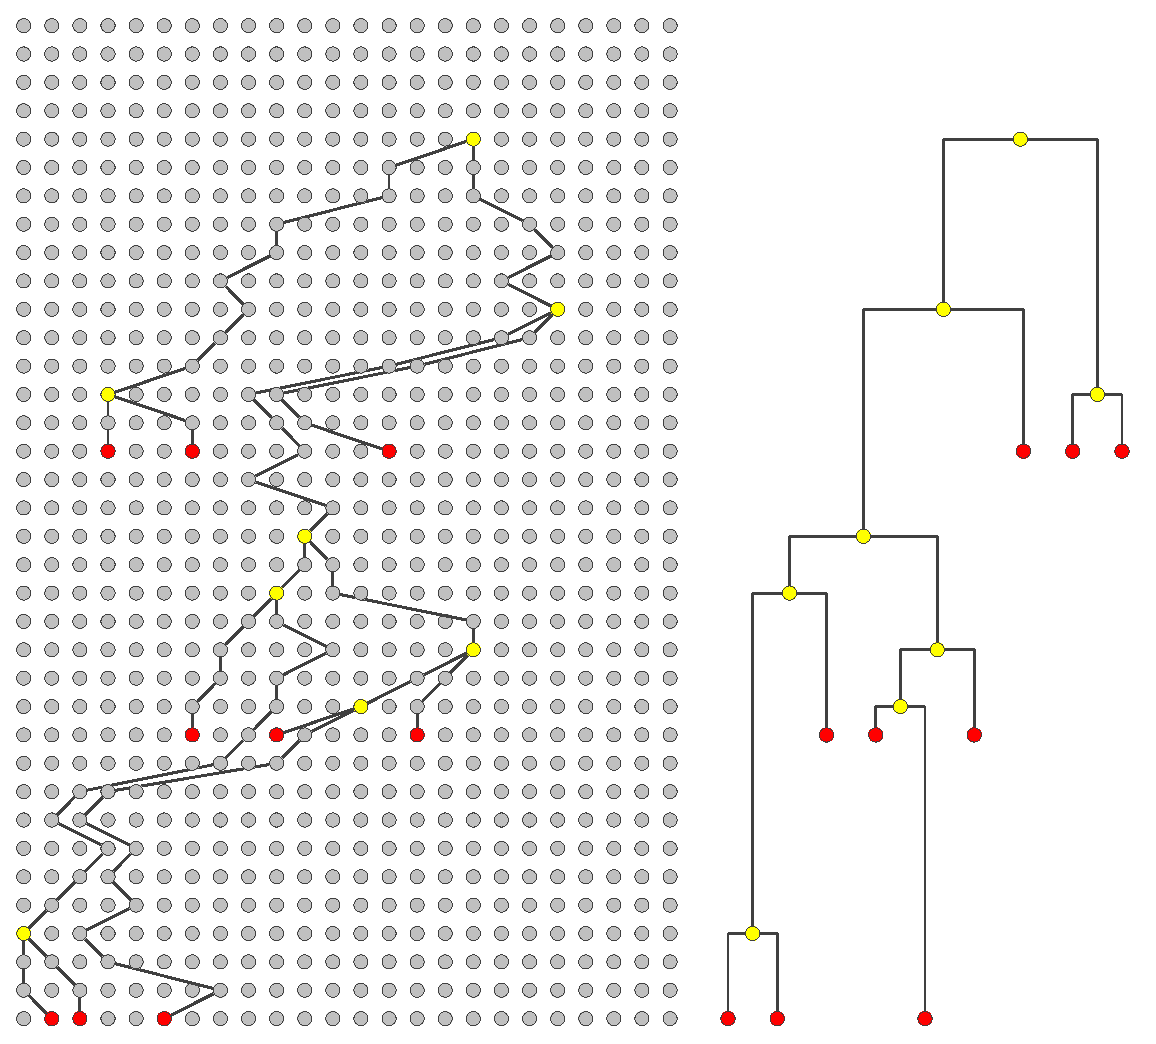
\includegraphics[width=\textwidth]{../images/serialConstant}%

\center{
Constant size}

\column{0.5\textwidth}

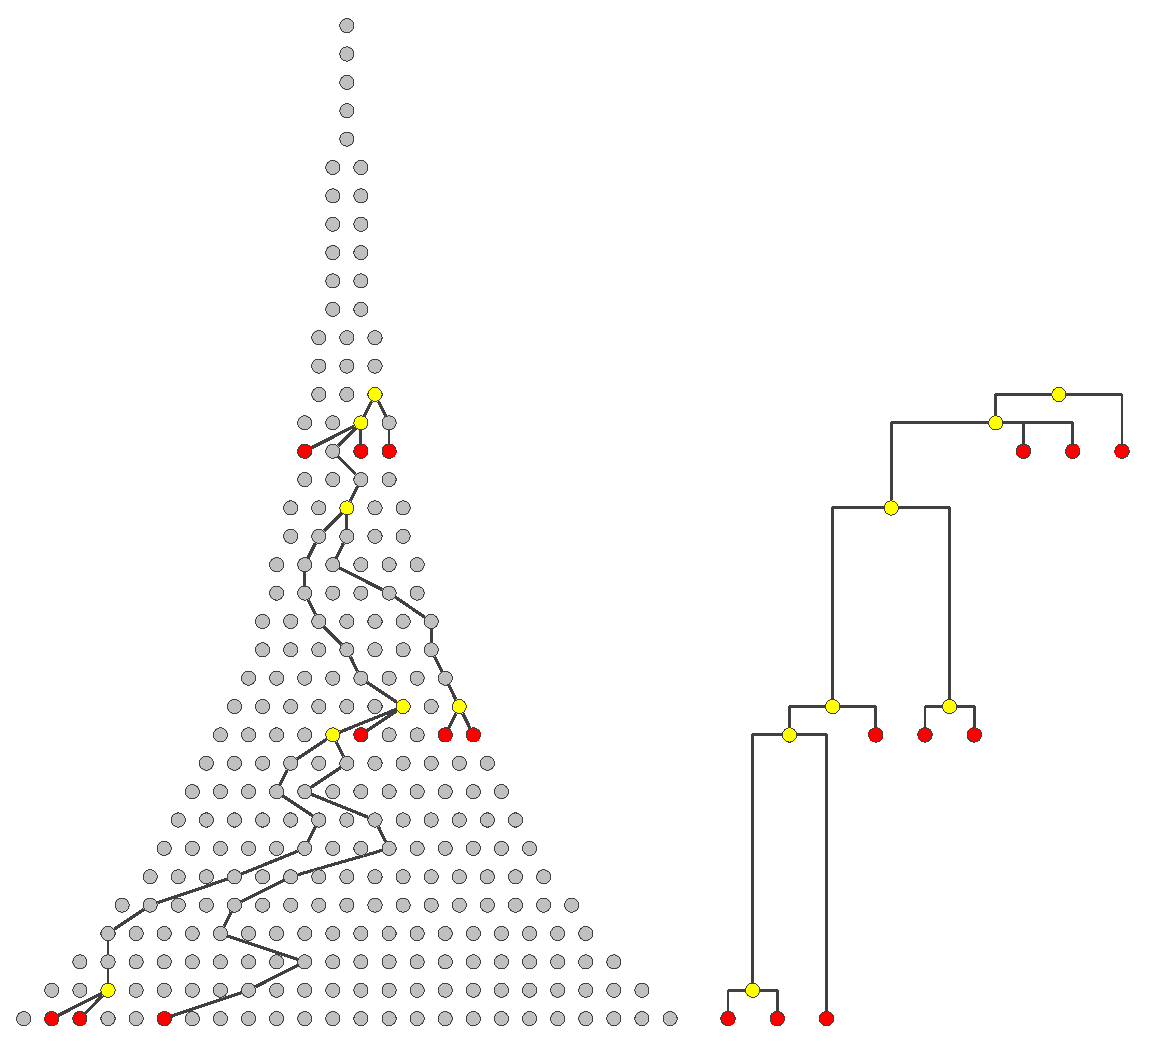
\includegraphics[width=\textwidth]{../images/serialExponential}%

\center{
Exponential growth}

\end{columns}

\end{frame}

\begin{frame}
\frametitle{Bayesian integration of uncertainty in genealogies}

\center{
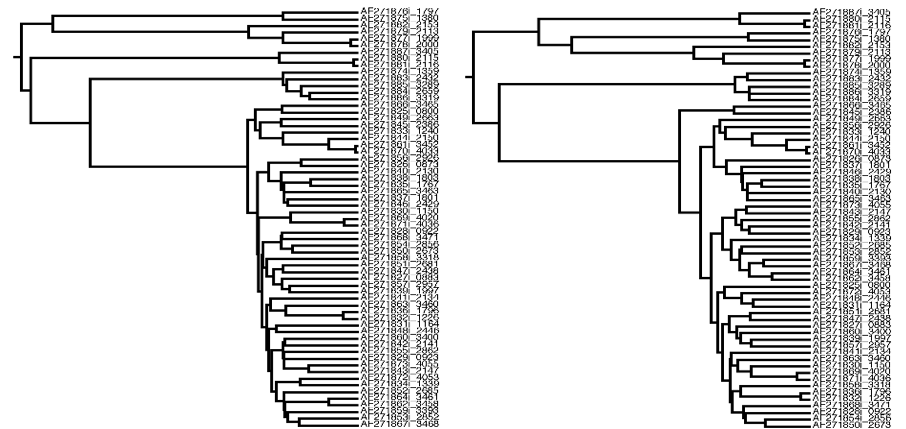
\includegraphics[scale=0.32]{../images/genealogicalUncertainty}
}

\smallskip

How similar are these two trees? Both of them are plausible given the data.
We can use Bayesian Markov-chain Monte Carlo to average the coalescent over all plausible trees.
\end{frame}
